
\section{Experimental Evaluation}\label{sec:exps_openwebtext}

In this section, we evaluate \SCONE in pre-training settings. In \cref{subsec:exp_gpt}, we assess \SCONE on GPT-2–sized models to study various design choices, and in \cref{sec:exps_dolma}, we extend the evaluation to large-scale pre-training scenarios involving trillions of tokens. Finally, in \cref{subsec:inference_cost}, we analyze the inference and storage costs during deployment.

For completeness, we also evaluate \SCONE in post-training settings by applying it during the SFT stage of recent Qwen3 models \citep{yang2025qwen3}; these results, presented in \cref{subsec:sft_qwen3}, show that \SCONE remains effective in post-training as well.


\subsection{Experiments with GPT-2}
\label{subsec:exp_gpt}

We analyze three key hyperparameters: (i) the maximum f-gram length $K$ in $\Vfgram$, (ii) the number of f-grams used, $|\Vfgram|$, and (iii) the $\Afgram$ model size. We use the released GPT-2 tokenizer, which has $|\Vtoken| = 50,\!257$, and train on the WebText dataset \citep{openwebtext}. The tokenized corpus  contains 9B training tokens, from which we extract f-grams using the method in \Cref{subsec:key_discovery}.

We consider three main model sizes with 76M, 340M, and 510M non-embedding parameters. Including the token embedding layer, the total parameter counts increase to 128M, 419M, and 589M, respectively. These models are either trained using only the token embedding layer as a baseline or with an additional $\Afgram$ when \SCONE is applied. We train all models for 80B tokens, roughly twice the number of training tokens used in \citet{radford2018improving}, to ensure that the baseline models approach convergence. For evaluation, we use the validation split of WebText and WikiText-103 \citep{merity2016pointer}, one of the largest downstream datasets in \citet{radford2019language}. Additional implementation details are provided in \Cref{subsec:webtext_details}.

\subsubsection{Varying the Maximum f-gram Length}\label{subsec:max_ngram_size}


We study the impact of varying the maximum f-gram length $K$ in $\Vfgram$. We vary $K$ from 2 to 8 while keeping the total number of f-grams fixed at 20M. As $K$ increases, the frequency cutoff, which is the minimum number of times an \ngram{n} appears in the training corpus to be included in $\Vfgram$, also increases. The cutoff is 7 when $K=2$ and 108 when $K=8$.

For each value of $K$, we evaluate (i) the model's perplexity and (ii) the average length of matched f-grams on WikiText-103. The results are shown in \Cref{fig:scale_max_ngram_size}. We find that evaluation perplexity rises between $K=2$ and $K=4$, after which it plateaus with some fluctuations. A similar trend is observed for the average match length, defined as the average length of the f-grams matched by \SCONE for each token in the evaluation set. The average match length also increases between $K=2$ and $K=4$ and then stabilizes.
This trend is likely because longer f-grams are rarer after frequency-based ranking. As a result, even when $K$ is larger, most selected \ngram{n}s remain short. Additionally, longer f-grams from the training corpus are less likely to match sequences in downstream data. Experiments on the WebText validation split (\Cref{subsec:more_exp_webtext}) show a similar trend, although the average match length continues to increase slightly longer, plateauing around $K=6$.


Considering these findings, for the experiments in the remainder of this paper, we set the maximum f-gram length to $K=5$ unless stated otherwise.


\subsubsection{Varying the Number of f-grams}


\begin{figure*}[t]
    \centering
    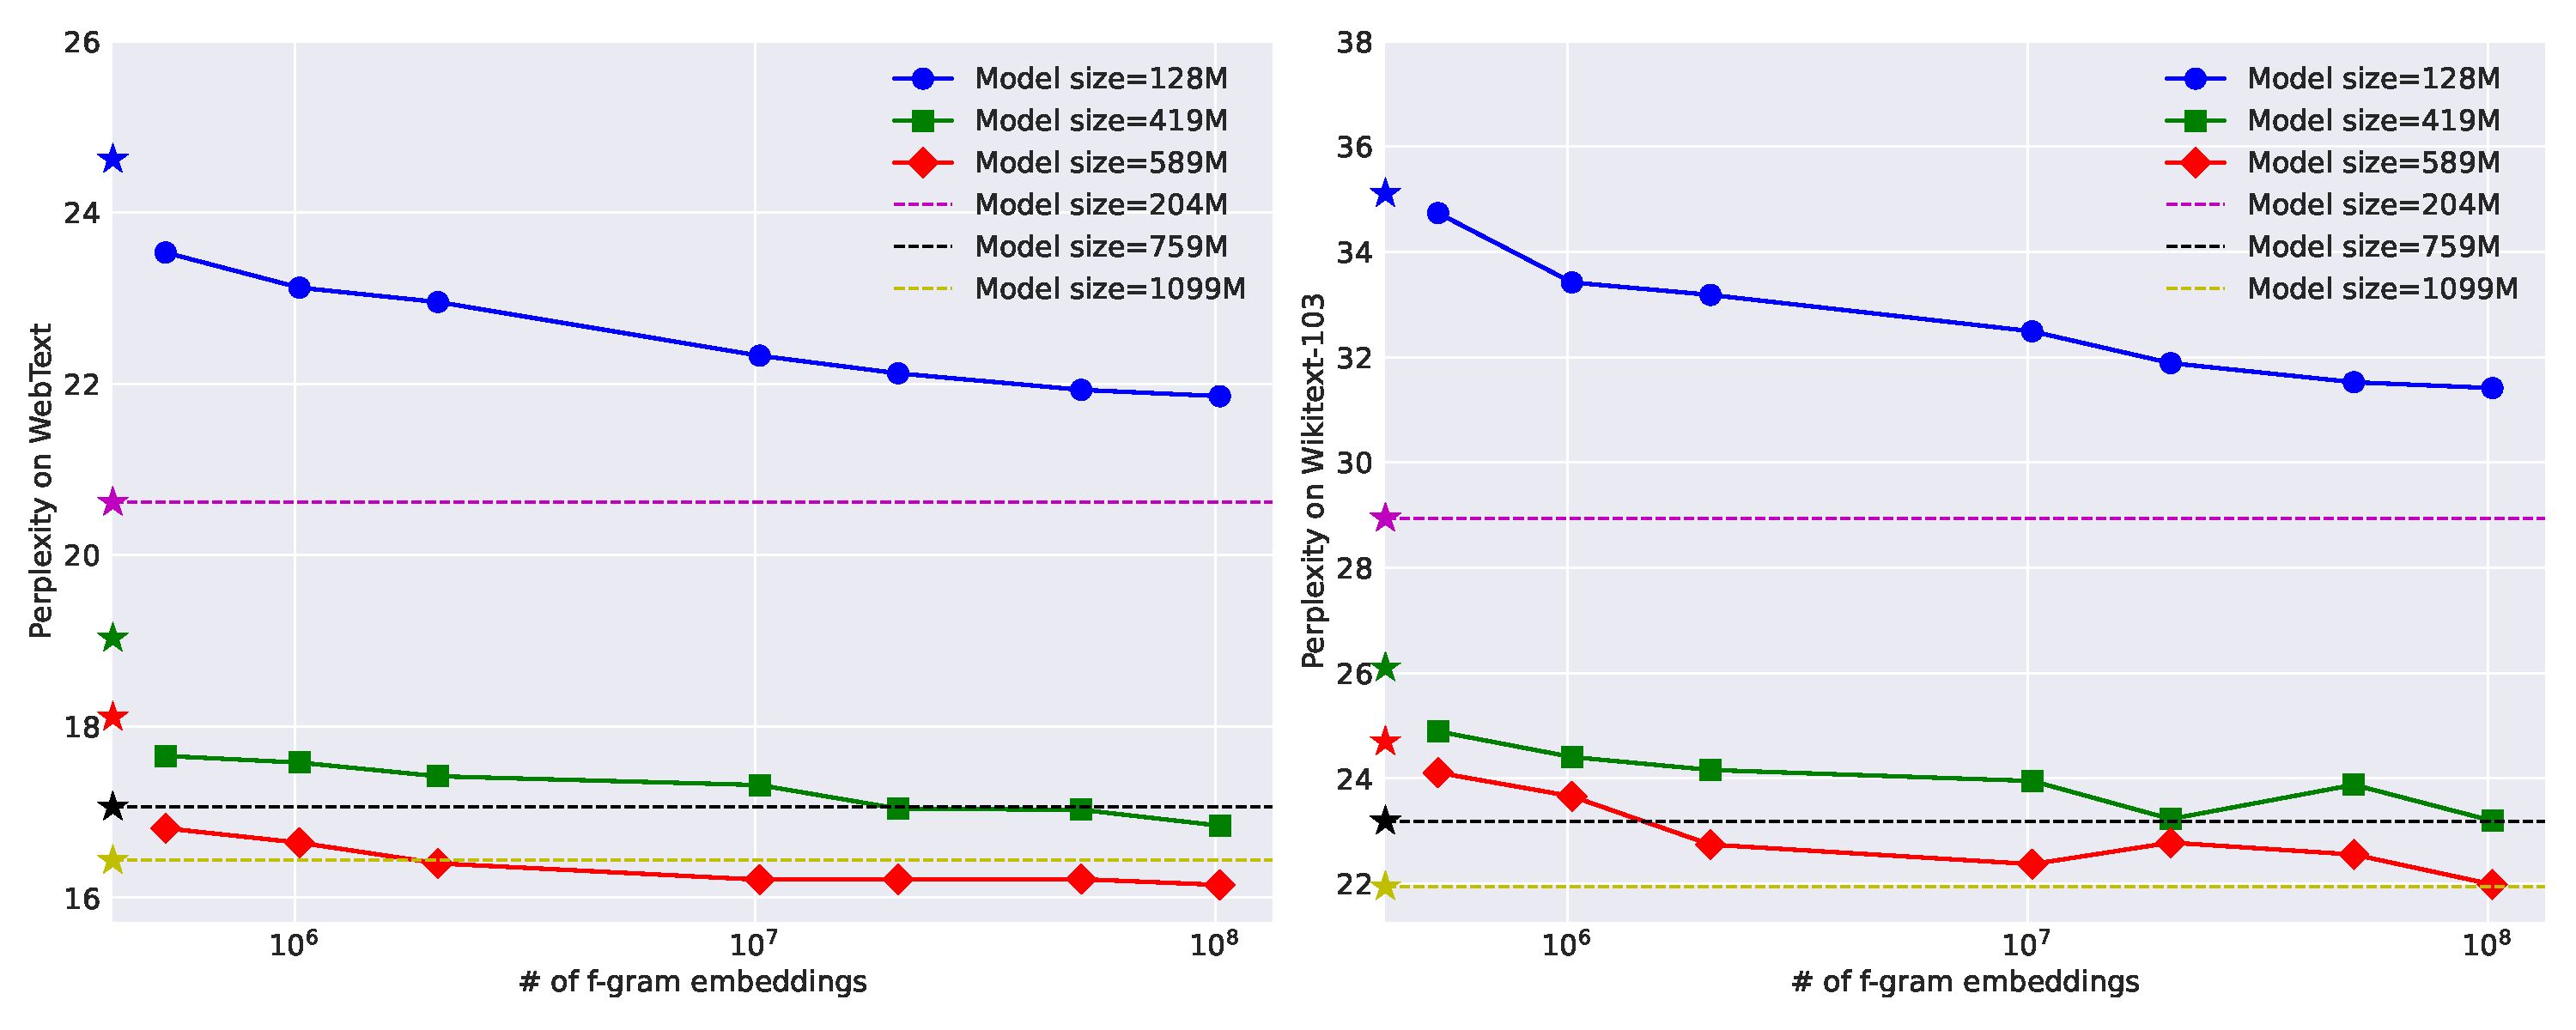
\includegraphics[width=0.8\linewidth]{figs/openwebtext_numgrams_eval_loss.pdf}
    \caption{Evaluation perplexity on WebText (left) and WikiText-103 (right) as a function of $|\Vfgram|$. Model sizes in the legend are number of parameters residing on the accelerator during inference. Dashed lines and leftmost stars show baseline performance. }

    \label{fig:scale_num_ngrams}
\end{figure*}



We observe consistent improvements in language modeling performance as we scale up $|\Vfgram|$.  To implement $\Afgram$, we replicate the baseline model architecture but remove the token embedding layer. This results in the size of $\Afgram$ matches the baseline model's non-embedding parameters. 

\Cref{fig:scale_num_ngrams} shows the evaluation perplexity as $|\Vfgram|$ increases from 512K to 100M. On the WebText validation split, the perplexity decreases consistently as the number of f-gram embeddings increases. Similarly, on WikiText-103, the perplexity generally decreases with more f-gram embeddings, though minor fluctuations are observed. 

In \Cref{fig:scale_num_ngrams}, we include three additional baselines where the non-embedding parameters of the three main models are doubled, resulting in models with 204M, 759M, and 1099M parameters for the original 128M, 419M, and 589M models, respectively. This ensures that the total parameter count of each baseline matches the training-time parameter count when \SCONE is applied. With 100M f-gram embeddings, the 419M and 589M models trained with \SCONE match or surpass the performance of the 759M and 1099M baselines, respectively, despite using only half as many non-embedding parameters during inference.


\subsubsection{Varying the Size of the $\Afgram$ Model}\label{subsec:ngram_model_size}


\begin{figure}[t]
  \centering
  \begin{minipage}{0.45\textwidth}
    \centering
    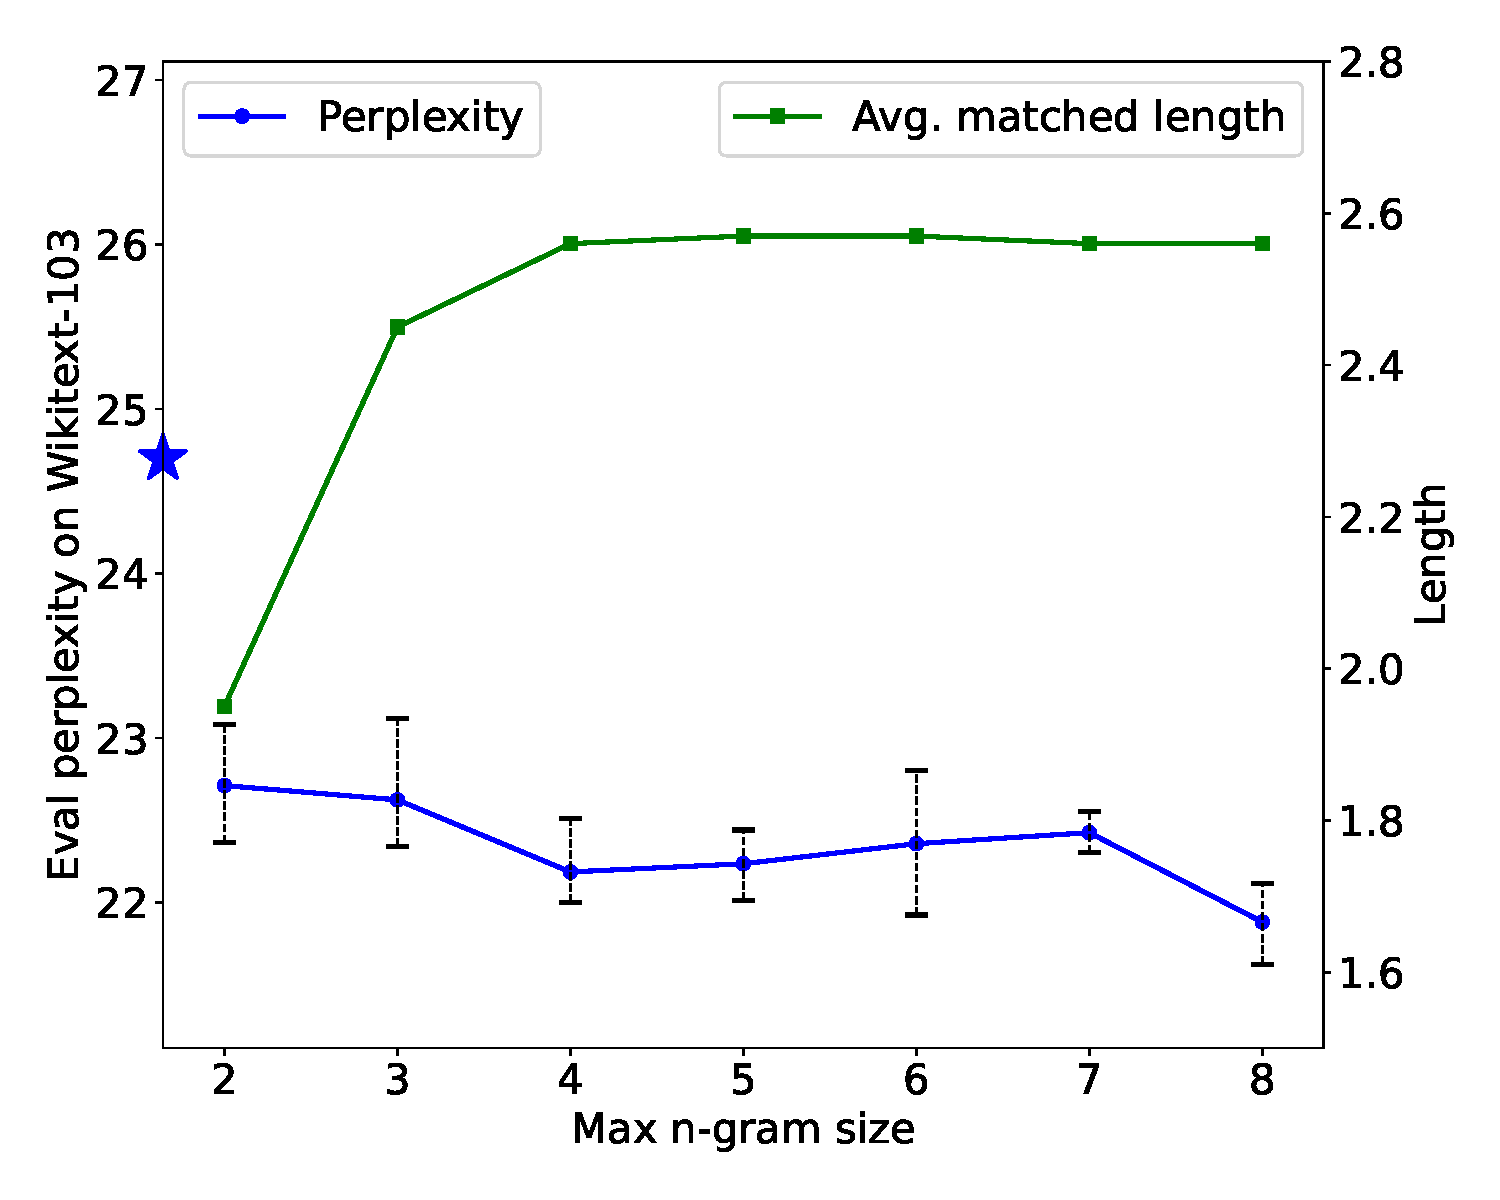
\includegraphics[width=\linewidth]{figs/openwebtext_maxngramsize_eval_loss_Wikitext-103.pdf}
    \caption{Effect of the maximum f-gram length $n$  on perplexity and matched length. Perplexity decreases as the maximum length increases from 2 to 4, then plateaus with minor fluctuations. Similarly, the average matched length stabilizes after length 4.}
    \label{fig:scale_max_ngram_size}
  \end{minipage}
  \hfill
  \begin{minipage}{0.48\textwidth}
    \centering
    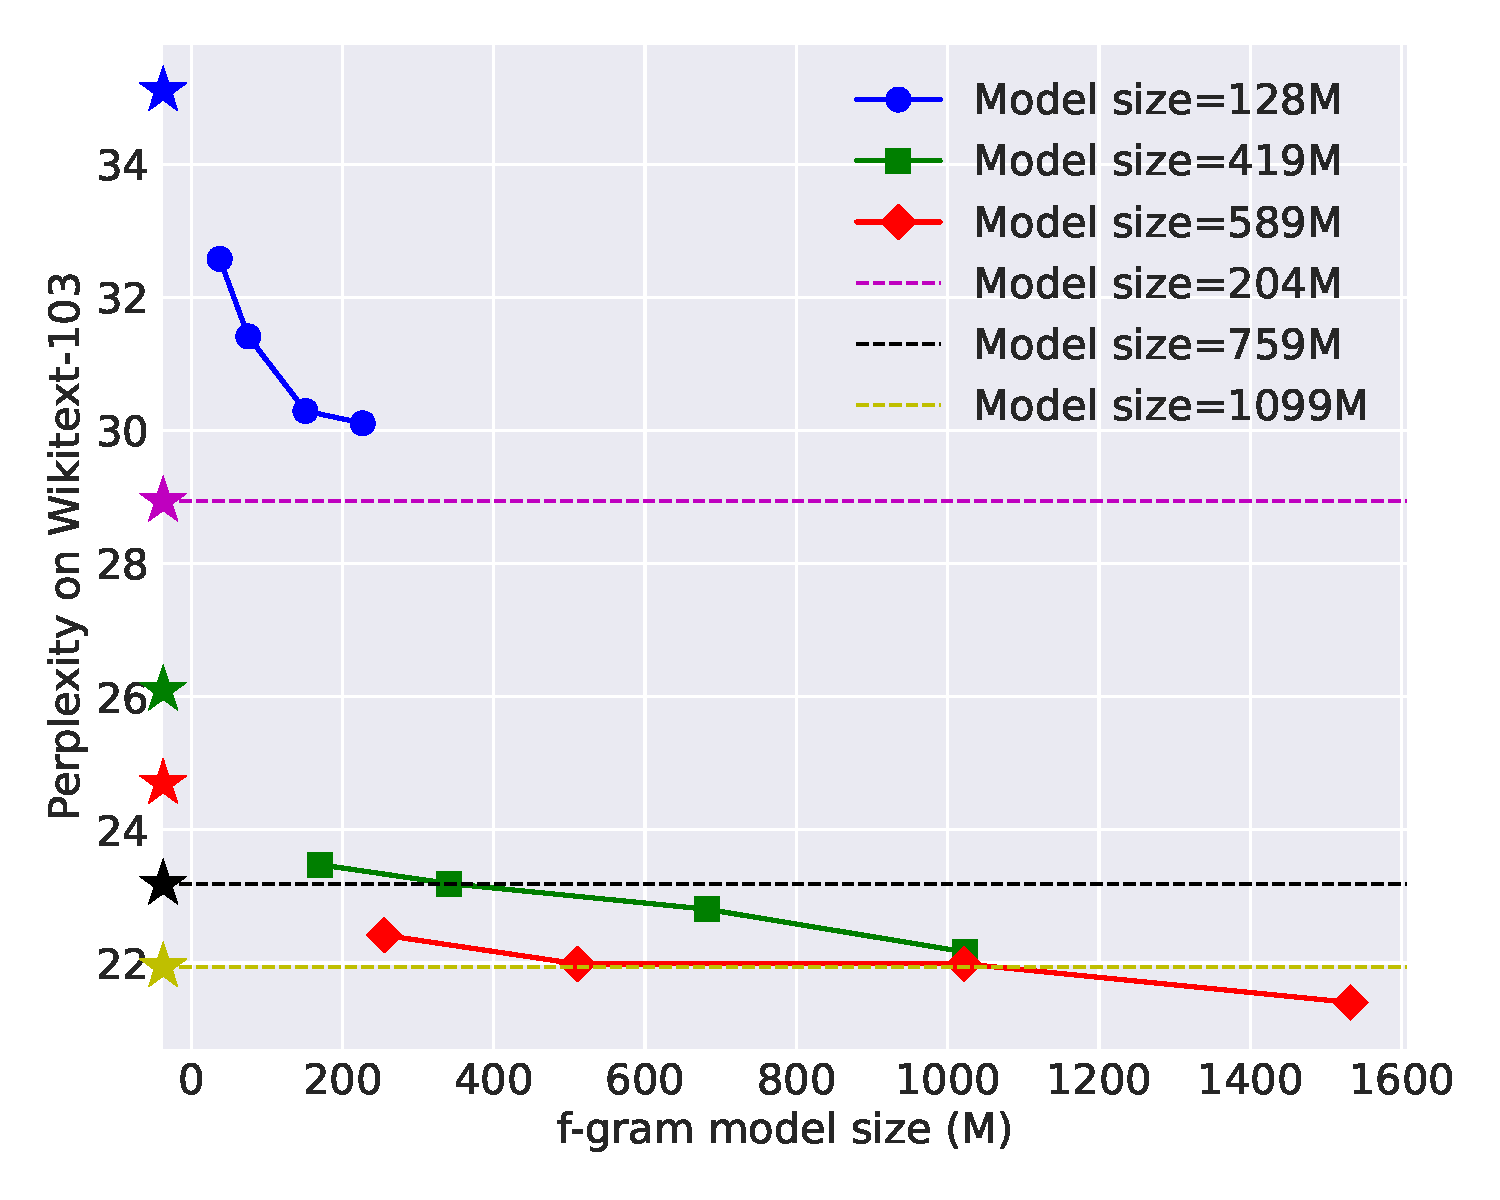
\includegraphics[width=\linewidth]{figs/openwebtext_ngrammodel_size_eval_loss_Wikitext-103.pdf}
    \caption{Evaluation perplexity improves as the size of $\Afgram$ grows. Model sizes in the legend are main model sizes, including the token embedding layer. Dashed lines and stars on the left represent baselines without an $\Afgram$ model.}
    \label{fig:scale_ngram_model}
  \end{minipage}
\end{figure}


We observe that, for a fixed $|\Vfgram|$, scaling up the $\Afgram$ model size provides a new way to improve language modeling performance. We vary the model size by changing the number of layers in the main model architecture. For each $\Amain$ model size, we evaluate four $\Afgram$ model sizes: 0.5x, 1x, 2x, and 3x the non-embedding parameters of the main model. We set $|\Vfgram|$ to be 100M. \Cref{fig:scale_ngram_model} presents the evaluation perplexity on Wikitext-103. The observations on WebText validation split are similar, and we present the results in \Cref{subsec:more_exp_webtext}.

The results in \Cref{fig:scale_ngram_model} show that the perplexity generally decreases as the $\Afgram$ model size increases, although the improvements become smaller as the model size grows larger. For instance, with the 419M main model, a 170M $\Afgram$ model improves the perplexity from 26.1 to 23.4, outperforming the 589M baseline (24.7) by a clear margin. Further scaling of the $\Afgram$ model to 1020M (resulting in 1439M total parameters during training) lowers the perplexity to 22.1, which is slightly higher than the 1099M baseline (21.9). This suggests that scaling up the $\Afgram$ model initially yields a better scaling curve, but beyond a certain size, it becomes less optimal compared to directly scaling up $\Amain$. However, scaling $\Amain$ also increases accelerator usage during inference, whereas scaling $\Afgram$ does not, since it is replaced with an off-accelerator lookup table at inference time. This highlights our method as a novel way to leverage additional training compute while maintaining fixed accelerator usage during inference.
